\begin{savequote}[75mm] 
The history of atomism is one of reductionism – the effort to reduce all the operations of nature to a small number of laws governing a small number of primordial objects.
\qauthor{Leon M. Lederman} 
\end{savequote}

\chapter{Laying the Foundation}


\newthought{This thesis represents a synergistic collaboration} between the worlds of High Energy Physics and Machine Learning. Using data originating from the European Center for Nuclear Research (CERN), we examine scalability and performance of novel Machine Learning methodologies on huge, high throughput datasets. A true instance of \textit{Big Data}, the CERN reads, stores, and analyses data at a rate of 25Pb per year, representing a challenge from a Machine Learning standpoint. Located on the border of France and Switzerland, the CERN is a multi-national collaboration comprised of multiple experiments, including ATLAS, CMS, LHCb, ALICE, and others.

The identification of subatomic particles within the ATLAS\footnote{A Toroidal LHC Apparatus} experiment is of the utmost importance for the discovery and verification of new physics phenomenon. In particular, many particle decays of importance to High Energy Physics result in jets associated with bottom ($b$) and charm ($c$) quarks. A jet is a cone-shaped stream of hadrons and other particles that are formed by the hadronization of a quark or gluon which shows up as energy deposits within the detector apparatus. Two very important analysis groups -- Higgs and Supersymmetrc searches -- use the identification of $b-$ and $c-$jets to identify relevant signal within search samples. A decay of the Higgs Boson to two bottom-like particles, $H \longrightarrow b\bar{b}$, uses so-called $b$-tagging to purify samples that only decay to a $b\bar{b}$ system. On the Supersymmetry side, so-called $c$-tagging is used to purify the search for the stop quark -- the supersymmmetric partner to the top quark. The stop quark undergoes a decay to a charm jet and a neutralino, $\tilde{t}\longrightarrow c + \tilde{\chi}_{1}^{0}$, and $c$-tagging can be used to probe this search further. The background of these searches -- searches who view Bottom or Charm jets as signal-- is primarily a mixture of Up, Down, and Strange quarks -- collectively referred to as \textit{light jets}.

\section{$b$-tagging}

Bottom quarks play a crucial role in most physics searches. Many high-energy particles decay into $b$-jets, thus, bottom jet reconstruction post hadronization can shed much light on the true decay chains of particles detected in the apparatus. Fortunately, Bottom Jets have unique identifying features that can be exploited by any algorithm. Hadrons containing bottom quarks have a long-enough lifetime that they travel some distance within the detector before decaying. On the other hand, their lifetimes are not so high as those of light quark hadrons (and associated), so they decay inside the detector rather than escape. The advent of precision silicon detectors within particle detectors has made it possible to identify particles that originate from a different place where the bottom quark was formed (e.g. the beam–beam collision point in a particle accelerator), and thus indicating the likely presence of a $b$-jet. Many so-called \textit{vertexing} variables lend themselves to any ma

\section{$c$-tagging}

Traditional binary discriminants on variables do not hold merit for $c$-tagging, as no variables produce adequate purity in signal to background ratio. To develop a well tuned, reliable $c$-tagger, we look to methods and frameworks that allow for arbitrary non-linear recombinations of variables, as any discrimination power will have to come from a non-linearly extracted basis. Most discriminants provide adequate separation between bottom and light jets, but no variables provide any separation for charm jets, making the proposition of charm tagging daunting.\\


\section{Data}
Training any classifier at ATLAS presents a unique scenario -- seemingly unlimited training data. Physicists understand the Standard Model of Particle Physics well enough to determine probabilities over decay channels, which means that simulations of particle can be constructed. Monte Carlo Generators are used to simulate particle collisions and the manner in which particles themselves interact with the detector apparatus. 

In most scenarios, this is ideal for any classification algorithm. However, two very unique issues present themselves in ATLAS data. Monte Carlo generated data does not perfectly model data from real beam collisions, and thus, over-training presents an unusually large risk, as we may over-train to relationships that are present in simulated data but not in data collected from the detector. Secondly, variables must be used whose distribution can differ between training and testing data. Any high energy physics classifier must use information from the transverse momentum (henceforth refered to as $p_{T}$
 ) and the pseudo-rapidity (referred to as $\eta$
 ), as these variables contain important information about the energy of the daughter particles. However, the kinematic combination of ($p_{T}$,$\eta$)
  is referred to as physics dependent -- meaning that all parameters of the distribution are dependent upon the decay channel taken. Thus, a large part of pre-training and training is taking measures to avoid over-fitting to a particular kinematic distribution.
  
\section{Mathematical Preliminaries}
This thesis makes heavy use of Linear Algebra. As such, we introduce notation to make concepts more legible and to err on the side of being mathematically brief. I begin with a general overview of notation to pull the reader into the symbolical semantics of this thesis. 

In general, and unless otherwise noted, a capital letter, such as $A$, will represent a matrix, and $A^T$ will represent its transpose. A lower case letter, such as $a,b,c,x,y$, etc. will represent a scalar, with its un-italicized, bold-faced complements $\mathbf{a},\mathbf{b},\mathbf{c},\mathbf{x},\mathbf{y}$, etc. representing vectors. $A\mathbf{x}, AB, \mathbf{a}^T \mathbf{b}$, and $\mathbf{a} \mathbf{b}^T$ represent the standard matrix-vector, matrix-matrix, inner-product, and outer-product computations respectively.

Let $A\odot B$ represent the standard element-wise Hadamard Product between two matrices (or vectors) of identical dimension. Suppose we have a function $\varphi : \R \longrightarrow \mathbb{R}$, and a matrix/vector $A$. Then we say that $\varphi(A)$ is defined, and is simply the function $\varphi$ applied element-wise to the matrix/vector $A$.

Let $\mathbf{x}$ be some vector, and let $C=\{ (A_i,b_i) \}_{i=1}^{n}$ be some (clearly finite) collection of pairs of arbitrarily sized matrices and vectors. We ensure that the pairs satisfy

\begin{equation}
\label{condition on dimensions}
A_i \in\R^{p\times q} \Longleftrightarrow b_i\in\R^{p}, \forall p,q\in\N
\end{equation}

for all $i$. Now, we also need that the product

\begin{equation}
\label{condition on product}
(\prod_{i=n}^{1} A_i ) \mathbf{x}
\end{equation}


is defined. Then, let
\begin{equation}
\label{network_operator}
\boxtimes_{C}^{\varphi} ( \mathbf{x} ) \equiv  A_n \varphi( A_{n-1}\cdots \varphi(A_1 \mathbf{x}) \cdots )
\end{equation}


be the transformed, sequential product\footnote{This is the underlying operation in a neural network, so we provide a formalism and syntactical simplification.} over our collection $C=\{ A_i \}_{i=1}^{n}$. 

Consider a vector $(x_1,x_2,\ldots,x_n)=\mathbf{x}\in\R^{n}$. Define the softmax function over $\R$ to be 


\begin{equation}
\label{softmax}
\smax(x_i | \mathbf{x}) = \frac{e^{x_i}}{ \sum_{i = 1}^{n} e^{x_i} }
\end{equation}

Then, we simply say, given \eqref{softmax}, that 

$$ (\smax(\mathbf{x}))_i =  \smax(x_i | \mathbf{x})  $$

is the softmax transformation of the vector $\mathbf{x}$. We can note that given a vector, $\smax(\cdot)$ induces a probability distribution over it's elements -- i.e., $\sum_{i=1}^{n}x_i = 1$ and $x_i\in[0,1]\forall i$.

We also formalize our definition of a so-called \emph{sigmoid} function. For any $x\in\R$, we define its sigmoid mapping to $(0,1)$ to be 

\begin{equation}
\label{sigmoid}
s(x) = \frac{1}{1+e^{-x}}
\end{equation}

which has limits of 0 and 1 at $-\infty$ and $\infty$ respectively. We also "overload" \eqref{sigmoid} by saying that given a matrix or vector $A$, $s(A)$ is defined and is simply an element-wise application of $s(\cdot)$.

Let $s'(x)$ be the derivative of the sigmoid function. Conveniently, $s'(x) = s(x)(1 - s(x))$. We continue the abuse of overloading notation and say that for some matrix $A$, $s'(A) = s(A)\odot (1 - S(A))$.


%$$   B(A(\mathbf{x} + \delta\mathbf{x}) + \mathbf{a}) + \mathbf{b} = \mathbf{x}   $$






 









%For an example of a full page figure, see Fig.~\ref{fig:myFullPageFigure}.
%\begin{figure}  
%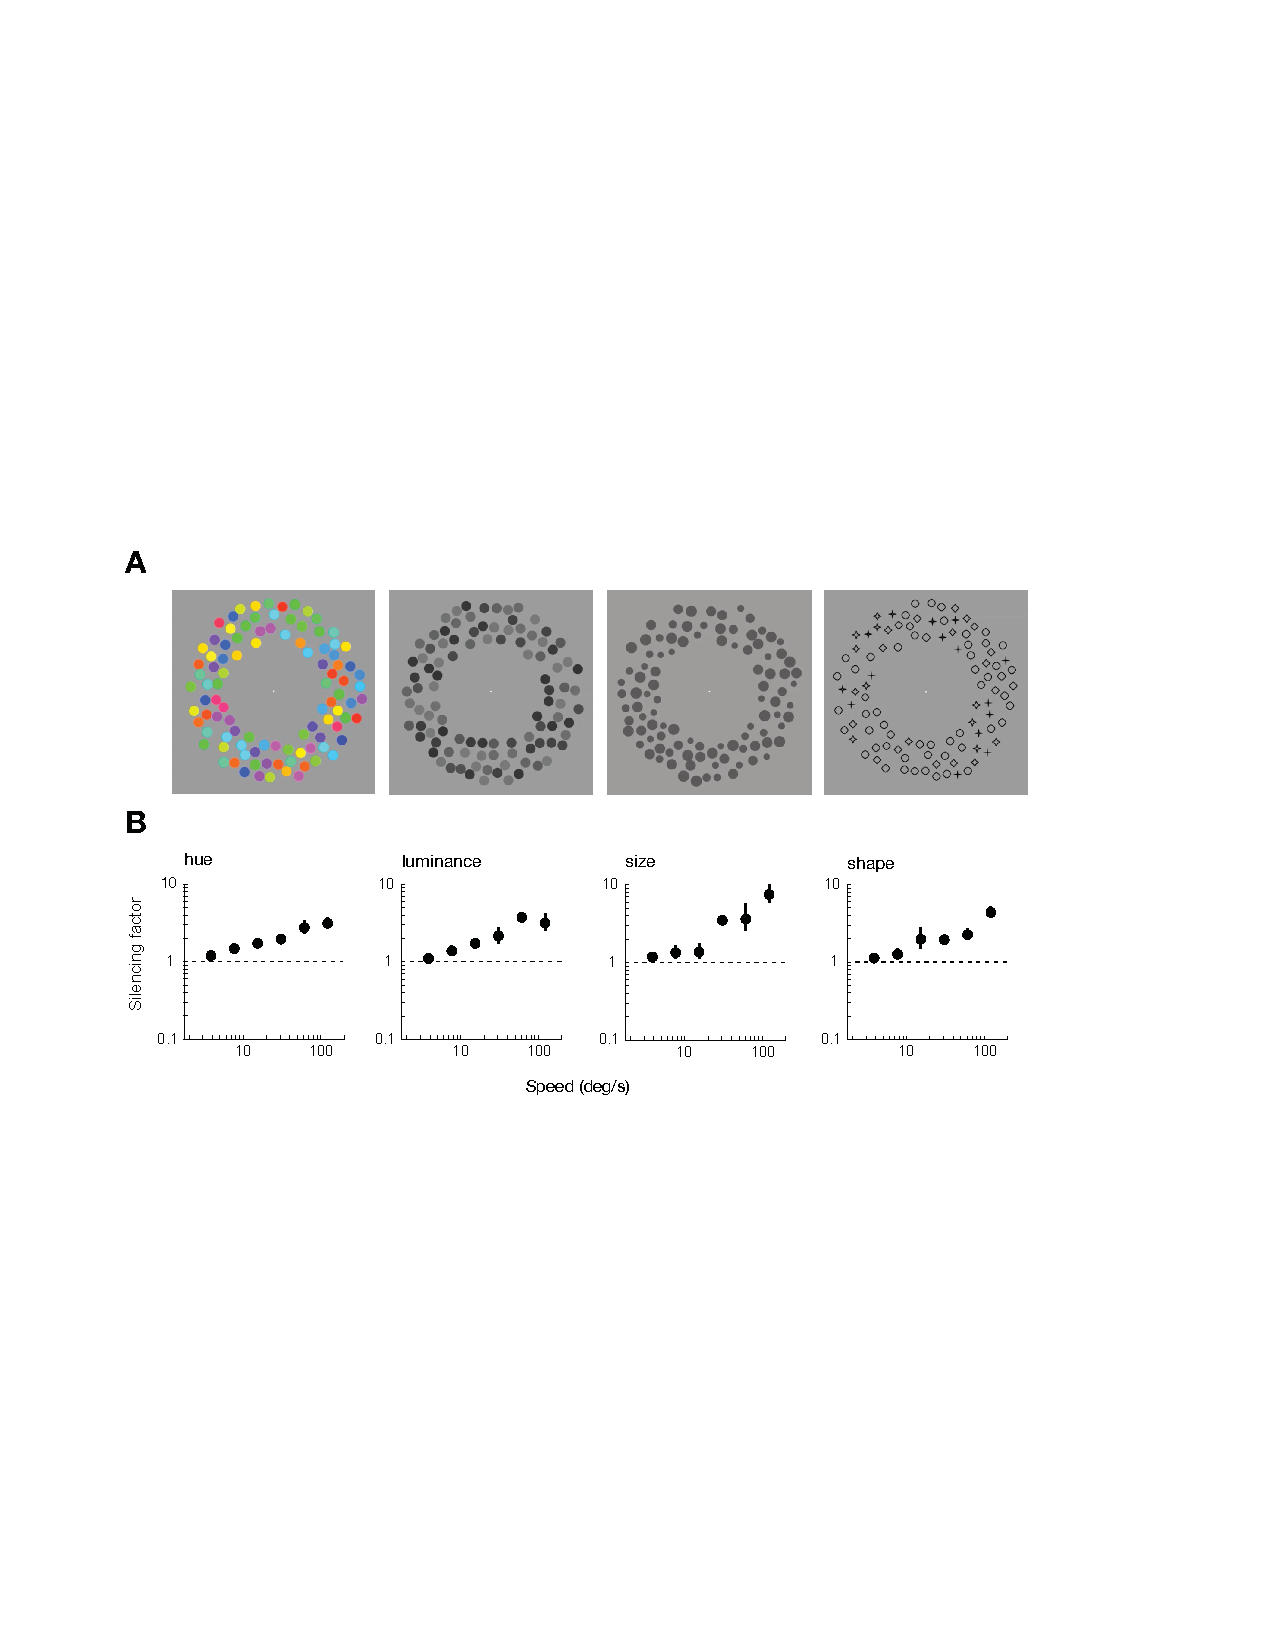
\includegraphics[width=\textwidth]{figures/fig1}
%\caption[Short figure name.]{This is a figure that floats inline and here is its caption.
%\label{fig:myInlineFigure}}
%\end{figure}


%\begin{FPfigure}  
%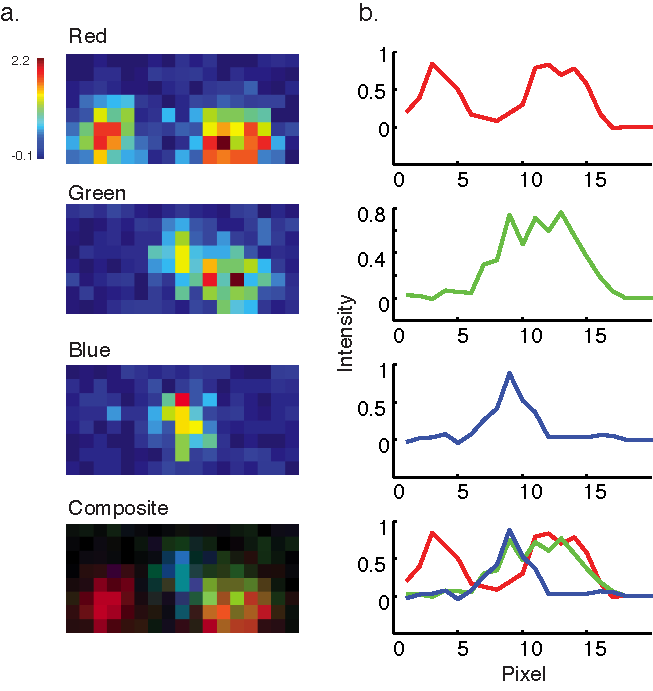
\includegraphics[width=\textwidth]{figures/fullpage}
%\caption[Short figure name.]{This is a full page figure using the FPfigure command. It takes up the whole page and the caption appears on the preceding page. Its useful for large figures. Harvard's rules about full page figures are tricky, but you don't have to worry about it because we took care of it for you. For example, the full figure is supposed to have a title in the same style as the caption but without the actual caption. The caption is supposed to appear alone on the preceding page with no other text. You do't have to worry about any of that. We have modified the fltpage package to make it work. This is a lengthy caption and it clearly would not fit on the same page as the figure. Note that you should only use the FPfigure command in instances where the figure really is too large. If the figure is small enough to fit by the caption than it does not produce the desired effect. Good luck with your thesis. I have to keep writing this to make the caption really long. LaTex is a lot of fun. You will enjoy working with it. Good luck on your post doctoral life! I am looking forward to mine. \label{fig:myFullPageFigure}}
%\end{FPfigure}
%\afterpage{\clearpage}

